\documentclass{article}
\usepackage[utf8]{inputenc}
\usepackage{graphicx}
\usepackage{xepersian}
\usepackage{fancyhdr}
\settextfont[Scale=1]{BNaznnBd.ttf}

\begin{document}
\pagenumbering{alph}
\tableofcontents
\clearpage
\listoffigures
\clearpage
\listoftables
\clearpage
\pagenumbering{arabic}
\lhead{}
\pagestyle{fancy}
\section{\lr{5g} چیست؟}
\lr{5g} خیلی خوبه خیلی خفنه خیلی بهمانه حالا بیاییم با \lr{4g} مقایسه کنیم. 
\begin{figure}[h]
\begin{center}
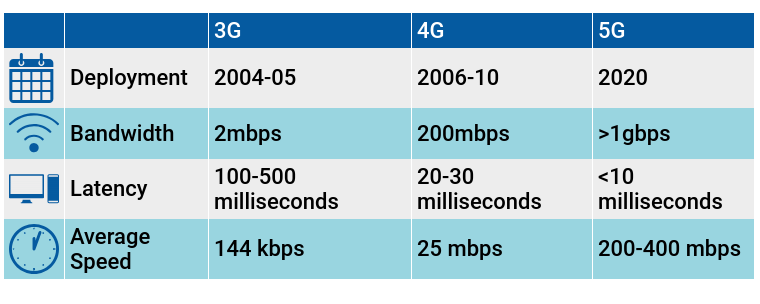
\includegraphics[width=9cm]{./3g-vs-4g-vs-5g.png}
\end{center}
\caption{مقایسه}
\label{image1}
\end{figure}
\\
حالا یه عکس\footnote{تصویر} دیگه را هم با هم ببینیم
\begin{figure}[h]
\begin{center}
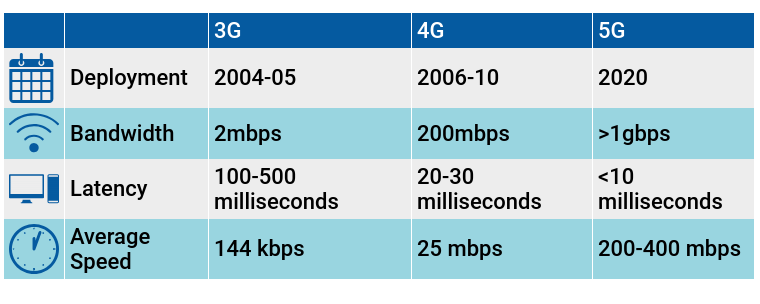
\includegraphics[width=9cm]{./3g-vs-4g-vs-5g.png}
\end{center}
\caption{مقایسه}
\label{image2}
\end{figure}
\newpage
اینجا هم در این قسمت یه رفرنس بزنیم به عکس یک 
  با دستور روبرو که در کد می بینید  \ref{image1}
\\
اینجا هم جدول داریم چه جدولی
\begin{table}[h]
\begin{center}


\begin{tabular}{||c c||} 
 \hline
 \lr{normalized required bandwidth} &\lr{HCM codeword} \\ [0.5ex] 
 \hline\hline
  $1$& $c_1,c_3,c_5,...,c_{N-1}$ \\ [2ex] 
 \hline
 $1/2$ & $c_2,c_6,c_1,....,c_{N-2}$\\[2ex] 
 \hline
  $\vdots$ & $\vdots$\\
 \hline
 $4/N $& $c_{N/4},c_{3N/4}$\\[2ex] 
 \hline
 $2/N $& $c_{N/2}$\\ [2ex] 
 \hline
\end{tabular}
\end{center}
\caption{پهنای باند هر کد}
\end{table}

\\
حالا نوبتی هم باشه نوبت فرمول نویسی هستش
 \begin{equation}
BER_{ACO} \approx \frac{\sqrt{M}-1}{\sqrt{M}\times \log_{2}(\sqrt{M})} \times erfc(\sqrt{\frac{3\times \gamma}{2(M - 1)}}) ;  \gamma = \frac{\alpha_{c}^2.\sigma^2}{\sigma_{N}^2 + \sigma_{c}^2}
\label{acober}
\end{equation} 


\end{document}
